% !TEX program = pdflatex
\documentclass[10pt,twocolumn]{article}

\usepackage[letterpaper,margin=0.68in,columnsep=0.24in]{geometry}
\usepackage[T1]{fontenc}
\usepackage{newtxtext,newtxmath}
\usepackage[scaled=0.92]{helvet}
\usepackage{courier}
\usepackage{microtype}
\usepackage{booktabs}
\usepackage{tabularx}
\usepackage{array}
\usepackage{graphicx}
\usepackage{xcolor}
\usepackage{enumitem}
\usepackage{amsmath}
\usepackage{siunitx}
\usepackage{tikz}
\usetikzlibrary{arrows.meta,positioning,fit}
\usepackage{pgfplots}
\pgfplotsset{compat=1.18}
\usepackage[numbers,sort&compress]{natbib}
\usepackage{xurl}
\usepackage{hyperref}
\usepackage[nameinlink,noabbrev]{cleveref}
\usepackage{fancyhdr}
\usepackage{titlesec}
\usepackage{caption}
\usepackage{balance}
\usepackage{listings}

\definecolor{MemiRuby}{HTML}{E5385D}
\definecolor{MemiInk}{HTML}{16171A}
\definecolor{MemiMuted}{HTML}{5D626C}
\definecolor{MemiGrid}{HTML}{D9DCE1}
\definecolor{MemiGreen}{HTML}{15845D}
\definecolor{MemiAmber}{HTML}{B87503}
\definecolor{MemiBlue}{HTML}{3469C7}
\definecolor{MemiRed}{HTML}{BD304B}

\hypersetup{
  colorlinks=true,
  linkcolor=MemiBlue,
  citecolor=MemiBlue,
  urlcolor=MemiBlue,
  pdftitle={DesignWorkBench v2: Constructing a Professional Design Benchmark for Coding Agents},
  pdfauthor={Sarvesh Chidambaram},
  pdfsubject={Benchmark construction, practitioner calibration, artifact contracts, and cross-harness evaluation}
}
\captionsetup{font=small,labelfont=bf}
\setlist{leftmargin=*,nosep}
\setlength{\parindent}{1em}
\setlength{\parskip}{0pt}
\titleformat{\section}{\large\sffamily\bfseries}{\thesection}{0.5em}{}
\titleformat{\subsection}{\normalsize\sffamily\bfseries}{\thesubsection}{0.5em}{}

\pagestyle{fancy}
\fancyhf{}
\fancyhead[L]{\scriptsize DesignWorkBench v2}
\fancyhead[R]{\scriptsize Chidambaram, 2026}
\fancyfoot[C]{\scriptsize\thepage}
\renewcommand{\headrulewidth}{0.2pt}

\newcommand{\code}[1]{\texttt{\small #1}}
\newcommand{\pass}{\textcolor{MemiGreen}{\textbf{VERIFIED}}}
\newcommand{\blocked}{\textcolor{MemiRed}{\textbf{BLOCKED}}}
\newcommand{\pending}{\textcolor{MemiAmber}{\textbf{PENDING}}}
\newcommand{\AuthorORCID}{not supplied}
\lstset{
  basicstyle=\ttfamily\scriptsize,
  breaklines=true,
  columns=fullflexible,
  frame=single,
  rulecolor=\color{MemiGrid},
  backgroundcolor=\color{black!2},
  xleftmargin=0.5em,
  xrightmargin=0.5em
}

% Generated by generate_paper_assets.py. Do not edit by hand.
\newcommand{\PaperDate}{29 July 2026}
\newcommand{\BenchmarkSchema}{2}
\newcommand{\BenchmarkTracks}{15}
\newcommand{\BenchmarkTasks}{300}
\newcommand{\PublicTasks}{60}
\newcommand{\PrivateTasks}{180}
\newcommand{\HoldoutTasks}{60}
\newcommand{\MinTaskMinutes}{30}
\newcommand{\MaxTaskMinutes}{165}
\newcommand{\MedianTaskMinutes}{90}
\newcommand{\NegativeControls}{18}
\newcommand{\RunnerProfiles}{8}
\newcommand{\VerifiedRunners}{3}
\newcommand{\PreparedFixtures}{60}
\newcommand{\VerifiedFixtures}{0}
\newcommand{\Practitioners}{0}
\newcommand{\CalibratedTracks}{0}
\newcommand{\MinimumPractitioners}{4}
\newcommand{\MinimumExternalPractitioners}{2}
\newcommand{\ArtifactsPerPractitioner}{5}
\newcommand{\RatingsPerArtifact}{2}
\newcommand{\OverallAlpha}{0.8}
\newcommand{\TrackAlpha}{0.67}
\newcommand{\HarnessConditions}{4}
\newcommand{\DevelopmentRepeats}{3}
\newcommand{\ReleaseRepeats}{5}


\begin{document}

\twocolumn[
\begin{@twocolumnfalse}
\begin{center}
{\sffamily\bfseries\LARGE DesignWorkBench v2\\[0.15em]
\Large Constructing a Professional Design Benchmark for Coding Agents\par}
\vspace{0.8em}
{\large Sarvesh Chidambaram}\\
{\small Memi Design, United States}\\
{\small ORCID: \AuthorORCID\quad$\vert$\quad Correspondence through
\href{https://github.com/memi-design/memi}{memi-design/memi}}\\
\vspace{0.6em}
{\small Research artifact version 1.0 \quad$\vert$\quad \PaperDate \quad$\vert$\quad
Benchmark schema \BenchmarkSchema}
\end{center}

\begin{abstract}
Benchmarks for coding agents commonly score tests, screenshots, or short
interactions. Professional design work additionally requires evidence
judgment, editable source, platform fidelity, accessibility, critique,
validation, and a handoff another practitioner can continue. We introduce the
construction protocol for DesignWorkBench v2, a multidisciplinary benchmark
that treats design as complete work rather than visual imitation. The frozen
foundation specifies \BenchmarkTasks\ task contracts across \BenchmarkTracks\
tracks, partitioned into \PublicTasks\ public development tasks,
\PrivateTasks\ private tests, and \HoldoutTasks\ rolling holdouts. Tasks span
\MinTaskMinutes--\MaxTaskMinutes\ minutes and bind expected artifacts,
runtime runners, provenance, negative controls, and discipline-weighted
rubrics. Functional acceptance, senior-practitioner quality, source trust, and
efficiency remain separate outputs. Calibration requires at least
\MinimumPractitioners\ qualified practitioners per track,
\MinimumExternalPractitioners\ external to the benchmark author, blinded
ratings, and chance-corrected agreement. The current artifact is deliberately
incomplete: \PreparedFixtures\ public fixtures are prepared but
\VerifiedFixtures\ are independently verified, \VerifiedRunners\ of
\RunnerProfiles\ runner profiles have reproducible evidence, and no
practitioner calibration has been collected. We also preregister a matched
baseline, Memi, Superpowers, and Everything Claude Code comparison without
inventing results. This paper contributes a falsifiable benchmark design and
readiness accounting, not a claim that Memi has reached senior-practitioner
performance.
\end{abstract}

\noindent\textbf{Keywords:} design benchmark; coding agents; professional
practice; practitioner calibration; artifact provenance; human evaluation

\vspace{0.8em}
\hrule
\vspace{1em}
\end{@twocolumnfalse}
]

\section{Motivation}

Screenshot similarity and unit tests capture useful but narrow properties of
an interface. They do not establish that an agent framed the right problem,
used trustworthy evidence, preserved an editable system, handled error and
recovery states, respected platform conventions, or left a usable handoff.
Design2Code combines automated and human evaluation for screenshot-to-code
generation \cite{si2025design2code}; WebArena emphasizes reproducible,
long-horizon interaction \cite{zhou2023webarena}; and BigLaw Bench shows the
value of practitioner-authored tasks, bespoke rubrics, negative criteria, and
separate work-product and source-trust scores \cite{harvey2024biglaw}.

Benchmark construction itself is a failure surface. SWE-bench Verified was
created after expert review removed tasks that were hard or impossible to
solve \cite{openai2024swebench}; a later audit reported test defects and
contamination that reduced its usefulness for frontier evaluation
\cite{openai2026swebench}. DesignWorkBench therefore treats fixture
verification, leakage controls, runner evidence, and benchmark evolution as
first-class research objects.

The benchmark asks:

\begin{enumerate}
  \item Can an agent complete an end-to-end professional assignment?
  \item Is the artifact functionally accepted in the required runtime?
  \item How close is the work to a qualified senior practitioner's deliverable?
  \item Are claims traceable to supplied evidence and editable source?
  \item When quality is non-inferior, what tokens, time, retries, tools, and
  human intervention were required?
\end{enumerate}

\section{Construction Principles}

\subsection{Separate outcomes}

The benchmark reports four non-substitutable outcomes:

\begin{description}[style=nextline]
  \item[Acceptance.] Deterministic build, runtime, interaction, integrity, and
  artifact checks.
  \item[Professional quality.] Blinded, rubric-based judgment calibrated
  against qualified working practitioners.
  \item[Source trust.] Traceability from consequential claims to supplied
  sources, decisions, and evidence.
  \item[Efficiency.] Tokens, latency, tools, retries, interventions, and
  verification coverage, evaluated only after quality non-inferiority.
\end{description}

The separation blocks three common shortcuts: treating a passing build as
expert design, treating a polished screenshot as working software, and
claiming cost savings after silently lowering quality.

\subsection{Evidence caps}

Scores are bounded by the strongest admitted evidence. Prompt-only claims are
capped at 25; implemented and tested work at 65; runtime-reproduced and
independently validated evidence may reach 100. A model cannot award itself
practitioner status. Missing evidence is recorded as missing rather than
imputed from another track.

\subsection{Frozen units and immutable receipts}

Each evaluation cell binds a task revision, fixture hash, repository revision,
runtime profile, model, provider, reasoning setting, condition revision,
artifact bundle, and trace receipt. Generated candidates are not promoted by
editing status fields. A separate reviewer recomputes the candidate hash and
issues an immutable receipt.

\section{Task Bank}

\subsection{Tracks and modes}

The task bank contains \BenchmarkTracks\ professional tracks:
product; graphic and brand; motion; spatial, AR, and VR; agentic; iOS and
SwiftUI; cross-platform mobile and Expo; Android and Compose; native design
kits; design systems; design engineering; service; content; interaction and
prototyping; and research and evidence.

Each track contains 20 contracts and five recurring work modes: critique and
diagnose, create, modify in context, validate and hand off, and capstone
recovery. The contracts range from \MinTaskMinutes\ to \MaxTaskMinutes\
(\MedianTaskMinutes-minute median) and require both discipline artifacts and a
decision log, execution trace, and handoff note.

\begin{figure}[t]
\centering
\begin{tikzpicture}
\begin{axis}[
  width=\columnwidth,
  height=4.9cm,
  ybar,
  bar width=7pt,
  ymin=0,ymax=65,
  xlabel={planned task duration (minutes)},
  ylabel={tasks},
  xtick=data,
  grid=major,
  grid style={draw=MemiGrid},
  tick label style={font=\scriptsize},
  label style={font=\scriptsize}
]
\addplot[fill=MemiRuby,draw=MemiRuby]
table[x=minutes,y=tasks,col sep=comma]{generated/durations.csv};
\end{axis}
\end{tikzpicture}
\caption{Task-duration distribution. Longer contracts test system changes,
cross-functional validation, and recovery rather than single-screen output.}
\label{fig:durations}
\end{figure}

\subsection{Splits}

The \BenchmarkTasks\ contracts are frozen as \PublicTasks\ public development,
\PrivateTasks\ private test, and \HoldoutTasks\ rolling holdout tasks. Public
tasks support implementation and reproducibility. Private tasks measure
generalization without exposing exact fixtures. Holdouts rotate quarterly to
limit prompt memorization and benchmark-specific tuning. Practice or public
work cannot be relabeled as private evidence.

\subsection{Artifact contracts}

Every task declares required input kinds, editable output kinds, runner
profiles, acceptance fixtures, and negative controls. Required artifacts are
not interchangeable. For example, a native task cannot be satisfied by a web
mock, a layered design task cannot be satisfied by a flattened image, and a
service-design task cannot omit offline operations and support channels.

\section{Rubrics and Negative Controls}

\subsection{Professional dimensions}

Track-specific weights sum to 100 across ten shared dimensions: problem
framing; evidence judgment; craft; interaction behavior; system and platform
fidelity; accessibility, safety, and ethics; technical runtime quality;
validation; handoff and collaboration; and critique and recovery. Shared
dimensions support comparison, while track weights preserve professional
differences. Native-platform references include Apple and Android quality
guidance \cite{applehig2026,androidquality2026}; web artifacts incorporate
WCAG 2.2 and field-oriented performance criteria
\cite{wcag2024,webvitals2026}; spatial tasks bind OpenXR-compatible evidence
\cite{openxr2026}.

The benchmark uses a geometric composite across claimed tracks. A high web
score cannot numerically conceal a failed native, spatial, motion, or source
trust result. Every track is also reported independently.

\subsection{Negative controls}

The manifest defines \NegativeControls\ named failure controls. They include
fixture tampering, fabricated evidence, hidden-test leakage, scope
substitution, unsupported user needs, flattened artifacts, unsafe motion,
spatial comfort failures, silent agent overwrites, non-native substitution,
single-platform proof, duplicate-component debt, polished front ends without
required state, placeholder content, happy-path-only prototypes, and
unsupported research claims.

Negative controls are not optional deductions added after a favorable score.
They can invalidate evidence, cap scores, or fail acceptance. Their role is to
represent the human correction cost of plausible-looking but unsafe or
unusable work.

\section{Runner and Fixture Evidence}

\subsection{Runner contracts}

Eight runner profiles define evidence for browser and desktop web, iOS or
visionOS Simulator, Expo on iOS and Android, Android emulator and Compose,
editable design artifacts, motion rendering, spatial/XR, and cross-discipline
artifact provenance. A runner is verified only when every evidence kind in its
contract is reproducible and hash-bound.

At this paper revision, browser/Playwright, motion rendering, and artifact
validation are \pass. The remaining five are \pending. Tool installation,
capability detection, or a screenshot alone does not verify a runner.

\subsection{Fixture promotion}

The public authoring pass produced \PreparedFixtures\ deterministic candidate
packs. All \VerifiedFixtures\ are independently verified. Promotion requires:
reproducible source assets; license or permission evidence; private-material
separation; matching hashes; complete artifact and runtime contracts; and a
clean-environment handoff reopen. Benchmark authors cannot self-approve their
own candidates.

\section{Practitioner Calibration}

Each track requires at least \MinimumPractitioners\ qualified practitioners,
including \MinimumExternalPractitioners\ external to Memi. Qualification and
conflicts are recorded per track. Each practitioner completes at least
\ArtifactsPerPractitioner\ frozen artifacts, and every artifact receives at
least \RatingsPerArtifact\ independent blinded ratings. Graders do not receive
the author, model, provider, harness condition, another rating, or aggregate
result.

Ratings contain dimension scores, rationale, acceptance, evidence level,
artifact hash, qualification reference, and start and completion times.
Disagreements above eight points require a third adjudicator while preserving
the original ratings. Interval-scale Krippendorff's alpha
\cite{hughes2021alpha} must reach \OverallAlpha\ overall and at least
\TrackAlpha\ in every claimed track. Current calibration contains
\Practitioners\ practitioners and \CalibratedTracks/\BenchmarkTracks\
calibrated tracks; professional certification is therefore \blocked.

\section{Cross-Harness Evaluation Protocol}

The committed protocol defines \HarnessConditions\ conditions: no repository
design harness, Memi 2.7, Superpowers, and Everything Claude Code. The Skills
CLI is classified as installation and discovery transport, not as a
performance condition. The protocol is \emph{preregistered and unexecuted}.

\begin{figure}[t]
\centering
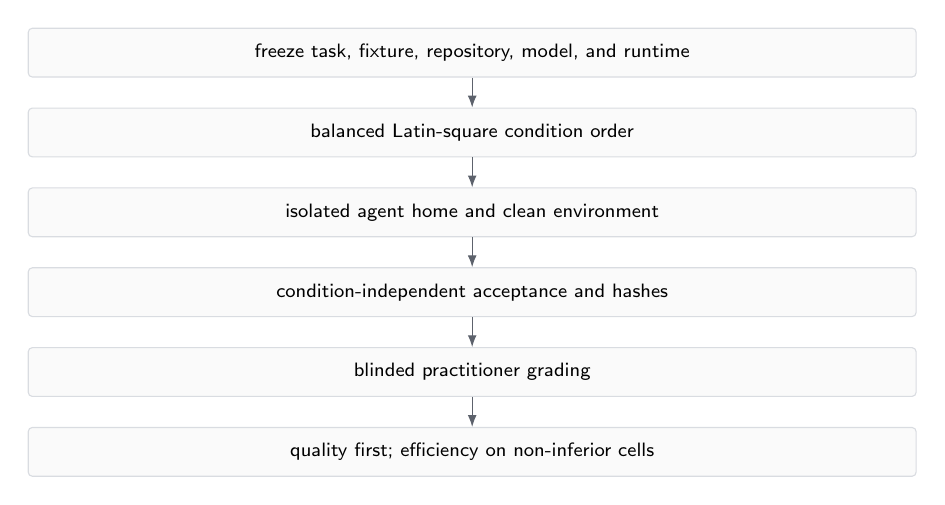
\begin{tikzpicture}[
  node distance=3.8mm,
  box/.style={draw=MemiGrid,rounded corners=1.5pt,fill=black!2,
    minimum width=0.93\columnwidth,minimum height=6.2mm,
    font=\sffamily\scriptsize,align=center},
  arrow/.style={-{Latex[length=1.5mm]},draw=MemiMuted}
]
\node[box] (freeze) {freeze task, fixture, repository, model, and runtime};
\node[box,below=of freeze] (order) {balanced Latin-square condition order};
\node[box,below=of order] (run) {isolated agent home and clean environment};
\node[box,below=of run] (verify) {condition-independent acceptance and hashes};
\node[box,below=of verify] (grade) {blinded practitioner grading};
\node[box,below=of grade] (report) {quality first; efficiency on non-inferior cells};
\draw[arrow] (freeze) -- (order);
\draw[arrow] (order) -- (run);
\draw[arrow] (run) -- (verify);
\draw[arrow] (verify) -- (grade);
\draw[arrow] (grade) -- (report);
\end{tikzpicture}
\caption{Predeclared cross-harness comparison. Conditions cannot select
different tasks, models, acceptance contracts, or graders.}
\label{fig:crossharness}
\end{figure}

The experimental unit is task--repository--model--repeat. Repository and task
revisions, fixture hash, model, provider, reasoning effort, context window,
permissions, network policy, runtime image, time limit, acceptance contract,
and grader blinding are held fixed. Condition order uses a balanced Latin
square. Development cells require \DevelopmentRepeats\ independent runs;
release-critical holdouts require \ReleaseRepeats.

Primary outcomes are acceptance, senior work-product score, source trust, and
critical defect count. Secondary outcomes are total and uncached tokens, wall
time, tool calls, retries, human interventions, and verification coverage.
Analysis is paired and stratified by track, with paired bootstrap intervals
and exact sign tests. A harness is ranked only after all admitted conditions
complete the same frozen cells and quality non-inferiority passes. Structured
authentication or setup failures are reported by cause, not converted into
performance zeros or wins for another condition.

\begin{table}[t]
\centering
\caption{Current cross-harness result status. Dashes are absent measurements,
not zero scores.}
\label{tab:harness}
\scriptsize
\begin{tabularx}{\columnwidth}{@{}Xrrr@{}}
\toprule
Condition & Admitted runs & Quality & Efficiency \\
\midrule
No design harness & 0 & -- & -- \\
Memi 2.7 & 0 & -- & -- \\
Superpowers & 0 & -- & -- \\
Everything Claude Code & 0 & -- & -- \\
\bottomrule
\end{tabularx}
\end{table}

\section{Current Readiness}

\begin{table}[t]
\centering
\caption{Foundation and certification are deliberately separate.}
\label{tab:readiness}
\scriptsize
\begin{tabularx}{\columnwidth}{@{}Xrrl@{}}
\toprule
Evidence unit & Prepared & Verified & Status \\
\midrule
Task contracts & \BenchmarkTasks & \BenchmarkTasks & frozen \\
Public fixture packs & \PreparedFixtures & \VerifiedFixtures & \blocked \\
Runner profiles & \VerifiedRunners & \VerifiedRunners & partial \\
Practitioners & 0 & \Practitioners & \blocked \\
Calibrated tracks & 0 & \CalibratedTracks & \blocked \\
Cross-harness cells & 0 & 0 & \blocked \\
\bottomrule
\end{tabularx}
\end{table}

The benchmark foundation validates structurally: \BenchmarkTracks\ tracks,
\BenchmarkTasks\ contracts, expected split counts, rubric totals, task hashes,
and runner contracts. This is not a quality score. It shows that the
measurement instrument is defined and machine-checkable. Certification
remains blocked on external work.

\section{Threats and Governance}

\textbf{Author involvement.} Memi authors designed the benchmark and may
benefit from its conclusions. External fixture review, blinded grading,
immutable negative evidence, and public protocols reduce but do not remove
this conflict.

\textbf{Construct validity.} Ten dimensions cannot exhaust every design
practice. Track rubrics and practitioner rationales must be reviewed after
calibration without retroactively changing frozen evaluations.

\textbf{Task realism.} The 60 public candidate packs are synthetic development
material. They are useful for deterministic tooling but cannot establish
ecological validity until independently verified and complemented by private
and holdout tasks.

\textbf{Provider and harness drift.} Models, harnesses, and dependencies
change. Every run pins versions, and comparisons may not mix revisions without
reporting them as separate conditions.

\textbf{Contamination.} Public tasks are assumed learnable. Private fixtures
are access-controlled, holdouts rotate, and leaked tasks are retired rather
than silently reused.

\textbf{Metric gaming.} Optimizing a geometric composite can still produce
artifacts that exploit rubric gaps. Negative controls, free-text practitioner
rationales, runtime evidence, and periodic adversarial audits are required.

Benchmark releases use semantic versions. Task edits change hashes; rubric or
split changes require a benchmark-version change; and results always identify
the benchmark, candidate, runner, and condition revisions.

\section{Reproducibility and Availability}

The benchmark manifest, public candidate fixtures, validation scripts,
runner receipts, calibration templates, preregistered cross-harness protocol,
paper source, generated tables, and readiness report are public
\cite{memibench2026,memireadiness2026}. Private and holdout fixtures are not
published. Public evidence retains content hashes so disclosed artifacts can
be verified without exposing protected source.

\begin{lstlisting}
npm run build:designwork-bench
npm run check:designwork-bench
npm run build:designwork-evidence
npm run check:designwork-evidence
npm run build:designwork-readiness
npm run check:designwork-readiness
npm run check:designwork-release
\end{lstlisting}

The ORCID field remains ``not supplied'' until the author provides a verified
identifier. This PDF is a research artifact and has not been peer reviewed.

\section{Conclusion}

DesignWorkBench v2 defines a benchmark for complete professional work:
discipline-specific artifacts, live runtimes, evidence trust, negative
controls, senior calibration, critique, recovery, and handoff. Its main
contribution is an evidence boundary that can refuse flattering conclusions.
The task bank and three runner profiles are reproducible; independent fixtures,
practitioner reliability, provider diversity, and matched cross-harness runs
remain incomplete. Those blocked cells are the next work, not numbers to infer.

\balance
\bibliographystyle{plainnat}
\bibliography{references}

\clearpage
\onecolumn
\appendix
\section{Runner Evidence Contracts}
\small
\begin{tabularx}{\textwidth}{@{}p{0.19\textwidth}p{0.19\textwidth}X@{}}
\toprule
Runner & Current evidence & Required evidence contract \\
\midrule
Browser and desktop web runtime & verified & browser-build, playwright-e2e, accessibility-tree, performance-trace \\
iOS or visionOS simulator runtime & pending & xcode-build, simulator-capture, accessibility-capture, performance-trace \\
Expo development and production runtime & pending & expo-build, ios-capture, android-capture, navigation-e2e \\
Android emulator and Compose instrumentation & pending & gradle-build, compose-ui-test, emulator-capture, accessibility-capture \\
Editable design artifact runtime & pending & layer-tree, component-graph, token-bindings, editable-export \\
Frame-accurate motion and video runtime & verified & timeline-source, render, frame-analysis, reduced-motion-output \\
Spatial simulator or OpenXR-compatible runtime & pending & scene-build, interactive-scenario, input-profile, comfort-safety-check \\
Cross-discipline artifact and provenance validator & verified & schema-validation, hash-verification, source-provenance, handoff-reopen \\
\bottomrule
\end{tabularx}


\section{Evidence Commitments}
\begin{tabularx}{\textwidth}{@{}X>{\ttfamily\tiny\raggedright\arraybackslash}p{0.49\textwidth}@{}}
\toprule
Artifact & SHA-256 \\
\midrule
\nolinkurl{benchmarks/designworkbench-v2/benchmark.json} & 69ebcc306e4751452e7dad12850f5be2b43d5186a9b3aa66e683339638cff9e9 \\
\nolinkurl{docs/audits/memi-designworkbench-v2-readiness.json} & 2c6cdfde67405664d32e4838ee5146de023e6e57df0abc77a9ddc1dc31e2939e \\
\nolinkurl{benchmarks/designworkbench-v2/PRACTITIONER_CALIBRATION.md} & 969f1853baf1006d24df961628ee33f695665e009f8949e6216d8824bda15f82 \\
\nolinkurl{benchmarks/designworkbench-v2/evidence/evidence.json} & 8c9fc9817f823827a76362bb6fee3aa2e5bed152d05d856ec6628ace7f99e012 \\
\nolinkurl{docs/research/designworkbench-v2-paper/cross-harness-protocol.json} & 9a5a9d51d58a0ad27db080bb08b167e5f92191006d64a2b02b3705eedc3cf22c \\
\bottomrule
\end{tabularx}


\section{Track Inventory}

\begin{tabularx}{\textwidth}{@{}llX@{}}
\toprule
Code & Track & Required discipline artifact families \\
\midrule
T1 & Product design & research synthesis, journey, IA, prototype, metrics \\
T2 & Graphic and brand & concept, identity system, compositions, production files \\
T3 & Motion & storyboard, timing system, animation source, render, reduced motion \\
T4 & Spatial/XR & spatial map, scene source, interaction model, safety evidence \\
T5 & Agentic design & authority model, state/trace UI, conflict and recovery flow \\
T6 & iOS/SwiftUI & native source, Simulator flow, accessibility, performance trace \\
T7 & Cross-platform mobile & Expo source, iOS/Android captures, navigation E2E \\
T8 & Android/Compose & Compose source, emulator flow, UI tests, accessibility \\
T9 & Native design kits & tokens, native components, platform mappings, usage guide \\
T10 & Design systems & tokens, components, governance, migration, adoption evidence \\
T11 & Design engineering & production source, states, tests, runtime, code handoff \\
T12 & Service design & research, blueprint, channel artifacts, operating model \\
T13 & Content design & evidence, content model, state copy, accessibility, governance \\
T14 & Interaction/prototyping & flows, state model, interactive source, usability evidence \\
T15 & Research/evidence & plan, corpus, analysis, findings, decision trace \\
\bottomrule
\end{tabularx}

\end{document}
